%%
%% Regular Expressions in Multi-typed Gene Expression Programming on the GPU.
%% The regex kingdom paper of the set; the shared material (the master symbol table,
%% the geneframe, the layout, the device-resident engine, HFF selection) is in the
%% core paper, cited as \cite{morgan_core}.
%%
%% Every measured number carries its source file in the text or in a table note.
%% Figures are drawn by pgfplots from papers/regex_multityped_gep_data/*.dat, which
%% were extracted from the phylu run logs named in each file's header.
%%
\documentclass[sigconf,nonacm]{acmart}

\usepackage{amsmath}
\usepackage{booktabs}
\usepackage{listings}
\usepackage{tikz}
\usepackage{pgfplots}
\usepackage{pgfplotstable}
\usepackage{xurl}
\pgfplotsset{compat=1.18}
\pgfplotstableset{comment chars={\#}}
\usetikzlibrary{arrows.meta,positioning,fit,shapes.misc}

\lstdefinestyle{mono}{basicstyle=\ttfamily\small, breaklines=true,
  columns=fullflexible, keepspaces=true}
\lstdefinestyle{rules}{basicstyle=\ttfamily\scriptsize, breaklines=true,
  breakatwhitespace=false, columns=fullflexible, keepspaces=true}
\newcommand{\rx}{\lstinline[style=mono]}
\newcommand{\ty}[1]{\textsf{#1}}
\newcommand{\sym}[1]{\textsf{#1}}
\newcommand{\src}[1]{{\small\nolinkurl{#1}}}

\begin{document}

\title{Regular Expressions in Multi-typed Gene Expression Programming on the GPU}
\subtitle{The POSIX regex kingdom: four types, a class algebra, and
Assertion Rule Golf evolved on the device}

\author{Andrew James Morgan}
\email{andrew@gamakon.ai}
\affiliation{%
  \institution{Gamakon Ltd.}
  \city{London}
  \country{United Kingdom}
}
\renewcommand{\shortauthors}{Morgan}

\begin{abstract}
We describe the regular-expression kingdom of a multi-typed Gene Expression
Programming (GEP) engine whose population, variation, expression and fitness
evaluation are resident on the GPU. The kingdom is a set of rows in the master
symbol table: nineteen POSIX-style operators over four value types
(\ty{Pattern}, \ty{CharClass}, \ty{Char} and an integer count \ty{I}), with a
class algebra of ranges, unions and negations, and counted repetition whose
operand is a class. Each type has its own head and tail in the gene, so every
genotype expresses a well-typed regular expression with no repair. On the device
the expressed tree is emitted, compiled to a Thompson virtual-machine program,
matched full-string against every row with a bit-set NFA, and scored as a
confusion matrix that hyperspherical fitness (HFF) reads; the fitness is Andrew
Morgan's Assertion Rule Golf, the search for a data-quality assertion rule from
labelled values. On one task, a UK-postcode detector (461 positive and 200
negative training values, scored on 198 unseen postcodes and 200 unseen
negatives), we report three measured stages of the kingdom. A single-type
alphabet reached 92.4\% held-out recall on one seed. The four-type alphabet with
a shared head reached 97.5\% on each of four seeds. The per-type layout
reached 100.0\% on each of four seeds at two program sizes, and counted
repetition, which the shared-head decoder could not draw on the device, appeared
in 18 of the 24 typed winners. No US ZIP, ZIP+4 or Canadian negative was accepted
in any of these runs. The comparisons are not single-variable: alphabet,
objectives and data split changed between the stages, and we set out each
difference. We also report the faults found while measuring, and the open work.
\end{abstract}

\maketitle

%% ============================================================================
\section{Introduction}
\label{sec:intro}

Enterprises keep the quality of their data with assertion rules: a column is
declared to hold UK postcodes, and a hand-written regular expression accepts the
values that are postcodes and rejects the rest. The rules are written and
maintained by people, and a column's name is often not a reliable guide to its
content. Andrew Morgan's hypothesis behind this kingdom is that if a regular
expression can be evolved by symbolic regression from labelled values, the
writing and maintenance of such rules can be automated from the data
alone~(\src{phylu/docs/PLAN_regex_evolution.md}, \S0). He calls the search
\emph{Assertion Rule Golf}: an assertion must partition the values correctly,
which is par, and among correct rules the cheapest to verify wins.

A regular expression is a typed tree. A character class is a set of bytes, a
range has two byte endpoints, a counted repetition has an integer count, and a
pattern is a sequence of the above. Classical GEP~\cite{ferreira2001gep} keeps
every offspring valid by admitting a single value type, so a regex in classical
GEP must either flatten these types into one, as our first alphabet did, or
reject and repair ill-typed trees. The multi-typed GEP core~\cite{morgan_core}
removes that restriction: a kingdom declares its types and its rows in the master
symbol table, the layout gives each type its own head and tail, and every
genotype expresses a well-typed phenotype. The regex kingdom was the first
kingdom with four genuinely distinct types and is the first real use of that
core.

This paper covers what is specific to the regex kingdom. The master symbol
table, the geneframe, the gene layout, the device-resident engine, HFF selection
and the pump are described in the core paper~\cite{morgan_core} and are not
repeated.

\paragraph{Contributions.}
\begin{enumerate}
\item The regex kingdom's rows: nineteen operators over four types, with a class
algebra and a counted repetition whose operand is a \ty{CharClass}, a choice that
makes the compiled program's length a bound fixed by the types
(Section~\ref{sec:kingdom}).
\item A device pipeline for the kingdom's fitness evaluation: an emit kernel from
the typed walk's nodes, a compile kernel that lowers a level-order tree to a
Thompson VM program in two linear passes without a stack, a bit-set NFA match
kernel over row bands, and a confusion-matrix scorer read by HFF, each checked
against a host reference and the \texttt{regex} crate
(Section~\ref{sec:gpu}).
\item Measurements of three stages of the kingdom on one task with retained logs,
data and seeds, with every confound between the stages stated
(Section~\ref{sec:experiments}).
\item An account of the faults found while measuring, including one that this
paper resolves: the zero rule length printed by every typed run
(Section~\ref{sec:faults}).
\end{enumerate}

%% ============================================================================
\section{Related Work}
\label{sec:related}

\paragraph{Typed genetic programming.} Strongly typed GP~\cite{montana1995stgp}
gives every argument slot a type and constrains the genetic operators to respect
them. GEP~\cite{ferreira2001gep,ferreira2006book} encodes a tree as a fixed-length
linear genome whose head and tail guarantee a valid tree under unchanged
operators, for one type. The core paper~\cite{morgan_core} sets out how the
master symbol table and the per-type layout carry that guarantee to many types;
the regex kingdom is one of its instances.

\paragraph{Evolving regular expressions.} Learning regular languages with GP
was studied by Svingen~\cite{svingen1998regular}. Bartoli et~al.\ evolve regular
expressions from examples with tree GP for text
extraction~\cite{bartoli2012regex,bartoli2016regex}; their target is a pattern
that extracts substrings, scored on character-level precision and recall. Our
target is a full-string assertion over a column, scored as a confusion matrix on
row labels, with selection by HFF. We have not compared against their system on
a common benchmark (Section~\ref{sec:limits}). Exact learning of regular sets
from queries and counterexamples is Angluin's $L^*$~\cite{angluin1987lstar}; it
needs an equivalence oracle, which a column of data does not supply.

\paragraph{Regex matching.} The compiled program and the matcher follow
Thompson's construction~\cite{thompson1968regex} and Cox's account of the
virtual-machine approach~\cite{cox2007regex,cox2009regexvm}: instructions
\textsf{Char}, \textsf{Split}, \textsf{Jmp} and \textsf{Match}, run as a set of
program counters advanced in lock step over the input, with no backtracking.
The running time is $O(|\text{program}|\cdot|\text{input}|)$ for every gene, which
is what makes the work of one fitness evaluation bounded on the device.

\paragraph{Simplification.} The kingdom's simplify editor rewrites a winner by
equality saturation in egglog~\cite{egglog}, with a contracting ruleset whose
rules each preserve the language. Brzozowski derivatives~\cite{brzozowski1964derivatives}
would decide equivalence exactly; we do not use them (Section~\ref{sec:limits}).

\paragraph{Masks.} The kingdom can match over Morgan's Data Quality on Read
(DQOR) masks~\cite{morgan2017bytefreq,morgan2017spark}, in which each character is
replaced by its class. The postcode runs reported here match raw values; the
mask path is described but not measured here.

%% ============================================================================
\section{The Kingdom}
\label{sec:kingdom}

\subsection{Types and rows}

The kingdom has four value types: \ty{Pattern} (a regex sub-tree, the root
type), \ty{CharClass} (a 256-bit set of bytes), \ty{Char} (one byte) and \ty{I}
(a repetition count). Its rows are \src{fuller/src/geneframe.rs}
\src{regex_rows} (lines 527--561), with one change made by the typed
kingdom, \src{fuller/src/regex_typed.rs} \src{typed_regex_rows}: the two
counted repetitions take a \ty{CharClass}, not a \ty{Pattern}.
Table~\ref{tab:rows} lists them. The constant-capable placeholders \sym{?\_Char}
and \sym{?\_I} are added by \src{typed_regex_relations}, and the optional
literal pattern terminal \sym{?\_Pat} defines a second variant of the kingdom.

\begin{table*}[t]
\caption{The regex kingdom's rows on the typed core
(\src{fuller/src/regex_typed.rs}). Arity is two at most.}
\label{tab:rows}
\small
\begin{tabular}{@{}llll@{}}
\toprule
row & spelling & inputs & output \\
\midrule
\sym{dot}, \sym{anchor\_start}, \sym{anchor\_end}, \sym{empty} & \rx!.! \rx!^! \rx!$! (empty) & --- & \ty{Pattern} \\
\sym{cc\_digit}, \sym{cc\_word}, \sym{cc\_space} & \rx!\d! \rx!\w! \rx!\s! & --- & \ty{CharClass} \\
\sym{star}, \sym{plus}, \sym{opt} & \rx!*! \rx!+! \rx!?! & \ty{Pattern} & \ty{Pattern} \\
\sym{concat}, \sym{alt} & $xy$, \rx!x|y! & \ty{Pattern}, \ty{Pattern} & \ty{Pattern} \\
\sym{rep\_n}, \sym{rep\_upto} & \rx!{n}!, \rx!{0,k}! & \ty{CharClass}, \ty{I} & \ty{Pattern} \\
\sym{class\_of} & a class as a pattern & \ty{CharClass} & \ty{Pattern} \\
\sym{lit} & one byte & \ty{Char} & \ty{Pattern} \\
\sym{cc\_range} & \rx![a-z]! & \ty{Char}, \ty{Char} & \ty{CharClass} \\
\sym{cc\_union} & set union & \ty{CharClass}, \ty{CharClass} & \ty{CharClass} \\
\sym{cc\_negate} & \rx![^...]! & \ty{CharClass} & \ty{CharClass} \\
\midrule
\sym{?\_Char} & a byte from $C_{\ty{Char}}$ & --- & \ty{Char} \\
\sym{?\_I} & a count from $C_{\ty{I}}$ & --- & \ty{I} \\
\sym{?\_Pat} (variant B only) & a byte from $C_{\ty{Pat}}$ & --- & \ty{Pattern} \\
\bottomrule
\end{tabular}
\end{table*}

The constant pools are data of the kingdom
(\src{fuller/src/regex_typed.rs} lines 32--43): $C_{\ty{Char}}$ and
$C_{\ty{Pat}}$ are the 95 printable ASCII bytes \texttt{0x20}--\texttt{0x7e} in
byte order, so a point mutation of a Dc index moves a literal to a neighbouring
byte, and $C_{\ty{I}}$ is the counts $0,\dots,8$, the compiler's clamp
(\src{MAX_REPEAT}, \src{phylu/src/evolve/regex_compile.rs:591}). A range's
endpoints are ordered by the compiler (\texttt{lo.min(hi)}, \texttt{lo.max(hi)},
\src{regex_compile.rs:628}), so every pair of bytes is a legal range.

\subsection{Legality by construction}

The kingdom passes the core's kingdom check (\src{KingdomContract::check}),
which derives, from the rows, the maximum arity of each type as a child of each
other type. For this kingdom
$a_{\ty{Pattern}}=a_{\ty{CharClass}}=a_{\ty{Char}}=2$ and $a_{\ty{I}}=1$, and the
heads for a program size $N$ (every program of up to $N$ functions) are
\[
h_{\ty{Pattern}}=2N-1,\quad h_{\ty{CharClass}}=h_{\ty{Char}}=2(N-1),\quad h_{\ty{I}}=N-1,
\]
asserted by the test \src{regex_bound_table} (\src{fuller/src/regex_typed.rs}).
Tails and Dc lengths follow from the per-producer bound of the core
paper~\cite{morgan_core}. Table~\ref{tab:layout} gives the two sizes measured
here. A head cell of type $T$ holds a row whose output is $T$; a tail cell holds a
terminal of $T$; a Dc cell holds an index into $C_T$. Initialisation, mutation
and crossover keep a cell inside its own type's alphabet, so the walk that
expresses a gene finds, at every slot, a symbol of the type that slot needs.
There is no fallback leaf and no repair: a gene that did not express would be a
defect of the software, reported as an error, and none occurred in the runs of
Section~\ref{sec:experiments}.

\begin{table}[t]
\caption{Gene layout per type at the two program sizes measured (from
\src{phylu/docs/PLAN_regex_on_typed_gep.md} \S2, computed by
\src{regex_bound_table}). $h/t/d$: head, tail and Dc lengths. Mutable
cells are $\sum (h+t)$, the figure the runs print; words add the Dc.}
\label{tab:layout}
\footnotesize
\setlength{\tabcolsep}{3pt}
\begin{tabular}{@{}rrrrrrrr@{}}
\toprule
$N$ & $L$ & Pat. & Class & Char & I & cells & words A/B \\
\midrule
12 & 46 & 23/24/-- & 22/45 & 22/45/46 & 11/12/23 & 204 & 273/319 \\
28 & 110 & 55/56/-- & 54/109 & 54/109/110 & 27/28/55 & 492 & 657/767 \\
\bottomrule
\end{tabular}
\end{table}

The 204 and 492 mutable cells are the figures printed by every run at those
sizes (\src{REGEX_TYPED} lines of \src{phylu/logs/REGEX_TYPED_AB/*.log}),
and the device profile reports 657 words a gene at $N=28$
(\src{profile_n28_v2.log}). The older shared-head gene of the same capacity
had 57 cells (head 28, tail 29).

\subsection{Counted repetition takes a class}

In the earlier four-type kingdom, \sym{rep\_n} took a \ty{Pattern} and was
expanded by copying its operand $k$ times. Nesting multiplies the copies:
$\sym{rep\_n}(\sym{rep\_n}(x,8),8)$ is 64 copies of $x$, so no fixed program
buffer holds every gene a layout can express, and a gene that overflowed would
have to be dropped, which the core forbids
(\src{PLAN_regex_on_typed_gep.md}, ``Decision: counted repetition takes a
CharClass''). In the typed kingdom the operand is a \ty{CharClass}. A class tree
of any size folds to one 256-bit set, so \sym{rep\_n} emits at most $k$
instructions and \sym{rep\_upto} at most $2k$, with $k\le 8$. The compiler's
buffers are then sized from the layout, never from a constant
(\texttt{capacity}, \src{fuller/src/regex_typed.rs}): at $N=12$ a gene has at
most 124 nodes and 393 instructions, at $N=28$ at most 300 and 937 (asserted by
\src{the_layout_bound_sizes_the_compiler}). The cost is expressiveness: a
repeated group such as $(ab)\{3\}$ must be written with \sym{star}, \sym{plus}
and \sym{opt}, which loop rather than copy. The formats the kingdom is for,
\rx!\d{3}! and \rx![A-Z]{1,2}!, are classes repeated.

\subsection{Two variants}

With the strict signatures a \ty{Pattern} tail holds only \rx!.!, \rx!^!,
\rx!$! and the empty pattern, so a single literal byte costs
$\sym{lit}(\sym{?\_Char})$: a function in the \ty{Pattern} head, a \ty{Char} cell
and a Dc index. Variant B adds \sym{?\_Pat}, a constant-capable \ty{Pattern}
terminal whose pool value is the byte it matches. Both variants are measured.

\subsection{Worked examples}

The rule evolved by the shared-head kingdom on seed 7013,
\rx!(?:[^X-t])+[^0-;]!, is the tree
\begin{align*}
\sym{concat}\big(&\sym{plus}(\sym{class\_of}(\sym{cc\_negate}(\sym{cc\_range}(\texttt{X},\texttt{t})))),\\
&\sym{class\_of}(\sym{cc\_negate}(\sym{cc\_range}(\texttt{0},\texttt{;})))\big).
\end{align*}
The class sub-trees fold to two sets; \sym{plus} emits its body and one
\textsf{Split}; the program is \textsf{Class}, \textsf{Split},
\textsf{Class}, \textsf{Match}: four instructions, the ``strokes 4/64'' of its
log (\src{phylu/logs/REGEX_POSTCODE_MT/run.log}). It reads ``one or more bytes
outside \texttt{X}--\texttt{t} (a range that holds \texttt{X}--\texttt{Z},
six punctuation bytes and \texttt{a}--\texttt{t}), then one byte that is not a
digit, a colon or a semicolon''.

A counted rule of the kind the typed kingdom can now draw,
\[
\sym{concat}(\sym{rep\_n}(\sym{cc\_range}(\texttt{A},\texttt{Z}),\sym{?\_I}{=}2),\,
\sym{class\_of}(\sym{cc\_digit})),
\]
prints as \rx!(?:[A-Z]){2}\d! and compiles to
\textsf{Class}, \textsf{Class}, \textsf{Class}, \textsf{Match}. The \ty{I}
operand is read from the \ty{I} head or tail and its Dc index from $C_{\ty{I}}$;
nothing in the gene can place a \ty{Pattern} in that slot.

\subsection{The earlier stages of the kingdom}

Two earlier alphabets were run on the same task, and the measurements of
Section~\ref{sec:experiments} compare them:

\begin{itemize}
\item \textbf{Single-type (stage S).} Nine \ty{Pattern} symbols (\rx!.!, \rx!\d!,
\rx!\w!, \rx!\s!, \rx!^!, \rx!$!, \sym{star}, \sym{concat}, \sym{alt}) and a
literal byte drawn as a random numerical constant (fuller \texttt{abffd8c6},
2026-10-04). No classes, no \rx!+!, no \rx!?!, no counts.
\item \textbf{Four types, shared head (stage P).} The nineteen rows of
Table~\ref{tab:rows} with \sym{rep\_n} taking a \ty{Pattern} (fuller
\texttt{51aa98d9}), decoded from one shared head by a total typed projection: a
token whose output type did not match the slot's demanded type was replaced by
that type's fallback leaf, and its subtree became non-coding. Counted repetition
was in the table and expanded by the host decoder, but the device decoder did
not expand it, so the search could not draw it
(\src{phylu/docs/reviews/2026-10-04_multityped_regex_result.md}, ``Honest
limits'').
\item \textbf{Four types, per-type layout (stage T).} This paper's kingdom
(phylu \texttt{0e69b7d4}, \texttt{8cc1cac6}, \texttt{3fd78355}).
\end{itemize}

%% ============================================================================
\section{Fitness Evaluation}
\label{sec:fitness}

\subsection{Assertion Rule Golf}

A dataset is a file of \texttt{value}\,TAB\,\texttt{label} rows, 1 for a value the
rule should accept and 0 for one it should reject
(\src{phylu/examples/regex_fit.rs}, \src{read_labelled}). A gene's rule is
matched full-string with byte semantics, as if written \rx!^(?:...)$!. The scorer
counts, per individual, the positives it rejects and the negatives it accepts,
and writes the rates into the score row HFF reads
(\src{phylu/src/evolve/regex_score.wgsl}):
\begin{gather*}
\textit{fn} = \frac{\text{positives rejected}}{n_{+}},\qquad
\textit{fp} = \frac{\text{negatives accepted}}{n_{-}},\\
\textit{len} = \frac{\min(n_{\text{inst}},64)}{64},
\end{gather*}
each on $[0,1]$, so HFF's caps are the identity. The first two are normalised by
their own class sizes so that the rarer class is not swamped. A rule with
$\textit{fp}=0$ is \emph{sound}: no bad value passes as good.

\subsection{The objective sets used in the runs}

The objective set changed between the builds measured, and this matters for
reading Section~\ref{sec:experiments}.

\begin{itemize}
\item \textbf{Stages S and P} (phylu \texttt{dfcbb1e2} and earlier): three HFF
objectives, \textit{fn}, \textit{fp} and \textit{len}, on all 661 training rows,
with no validation block (the run card of \src{REGEX_POSTCODE_MT} records
three HFF objectives; the build has no split).
\item \textbf{Stage T} (the current default,
\src{phylu/src/evolve/engine.rs:4490--4517}): the training file is split per
class, in file order, into 60\% train, 20\% validation and 20\% holdout
(\src{examples/regex_fit.rs:117--201}); for the postcode file this is 397, 132
and 132 rows. HFF reads eight columns: \textit{fn}, \textit{fp}, \textit{fn},
\textit{fp} on train and the same four on validation (the design lists the false
negative rate, false positive rate, $1-\mathrm{TPR}$ and $1-\mathrm{TNR}$, of which
the last two equal the first two, so each rate is counted twice). The rule-length
objective \textit{len} is \emph{off} by default since phylu \texttt{8b05aaa5}
(2026-10-05), because on the small mask alphabet it collapsed the population onto
a few short rules; it is restored by \src{EVOLVE_REGEX_PARSIMONY=1}, which no
stage-T run set. The holdout block is never scored on the device and is scored
once on the host at the end of a fit.
\end{itemize}

So stage T selected on train and validation error with no pressure on length,
and saw 529 of the 661 training rows; stage P selected on train error and length
and saw all 661. Both are scored afterwards on the same separate held-out file.

\subsection{Early stop}

A stage-T fit stops when its best individual has zero error on every HFF objective
and zero training \textit{fn} and \textit{fp} (\src{engine.rs:8784--8795}); the
holdout does not take part. \src{EVOLVE_REGEX_NO_EARLY_STOP=1} turns the
stop off, which the equal-budget arms use. Stages S and P had no early stop and
ran their full 180~s.

\subsection{Mechanisms not used in these runs}

The kingdom also has a signed ensemble (a chromosome of includer and excluder
genes, an excluder being a gene rooted at \sym{cc\_negate}), an evolved
per-gene active bit, a field selector for multi-field rows (raw value and masks),
a rejector sub-objective and false-positive weighting
(\src{regex_score.wgsl}; \src{engine.rs:4459--4535}). The postcode runs here use
one gene, one field, no signed fold and the default weight; on the typed core the
compile pass is given \texttt{n\_rnc = 0}, so every gene is active and reads field
0 (\src{PLAN_regex_on_typed_gep.md} \S7).

%% ============================================================================
\section{GPU Implementation}
\label{sec:gpu}

\subsection{The pipeline}

One generation runs variation, expression and fitness evaluation on the device
and reads the frame of results back to the host (Figure~\ref{fig:pipeline}).
Table~\ref{tab:where} states where each stage runs, with its source. The engine
around it (selection kernels, islands, the pump, HFF and TrueNorth) is the core
paper's~\cite{morgan_core}; only the five regex stages are specific to the
kingdom.

\begin{figure}[t]
\centering
\resizebox{\columnwidth}{!}{%
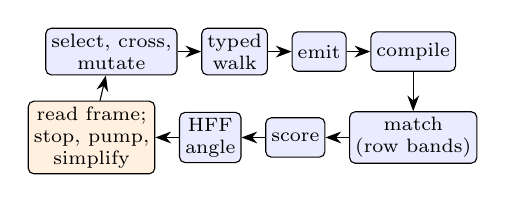
\begin{tikzpicture}[
  st/.style={draw, rounded corners=2pt, minimum height=5mm, font=\scriptsize, align=center, inner sep=2pt},
  dev/.style={st, fill=blue!8}, host/.style={st, fill=orange!12},
  ar/.style={-{Stealth[length=2mm]}}]
\node[dev] (vary) {select, cross,\\mutate};
\node[dev, right=3mm of vary] (walk) {typed\\walk};
\node[dev, right=3mm of walk] (emit) {emit};
\node[dev, right=3mm of emit] (comp) {compile};
\node[dev, below=5mm of comp] (match) {match\\(row bands)};
\node[dev, left=3mm of match] (score) {score};
\node[dev, left=3mm of score] (hff) {HFF\\angle};
\node[host, left=3mm of hff] (hostn) {read frame;\\stop, pump,\\simplify};
\draw[ar] (vary) -- (walk); \draw[ar] (walk) -- (emit); \draw[ar] (emit) -- (comp);
\draw[ar] (comp) -- (match); \draw[ar] (match) -- (score); \draw[ar] (score) -- (hff);
\draw[ar] (hff) -- (hostn); \draw[ar] (hostn) -- (vary);
\end{tikzpicture}}
\caption{One stage-T generation. Blue: compute kernels on the device. Orange: the
host, which reads the frame back each generation.}
\label{fig:pipeline}
\end{figure}

\begin{table*}[t]
\caption{Where each stage of a stage-T fit runs. Paths are in phylu
\texttt{src/evolve/} unless marked; line numbers are at phylu
\texttt{feat/shape-typed-kingdom} and fuller \texttt{feat/futhark-kingdom},
2026-11-01.}
\label{tab:where}
\footnotesize
\begin{tabular}{@{}p{0.34\textwidth}p{0.12\textwidth}p{0.5\textwidth}@{}}
\toprule
stage & runs on & source \\
\midrule
initial population and the pump's new individuals & device & \src{typed_init.wgsl} (\src{typed_init.rs:238}); \src{dev.init_rows}, \texttt{engine.rs:5076} \\
selection (elites, tournaments, cohort attributes) & device & \src{typed_select.wgsl} (\texttt{typed\_device.rs:32, :352}) \\
crossover, point mutation, constant mutation, cleanse & device & \src{typed_vary.wgsl} (\src{typed_vary.rs:914}); \texttt{dev.vary}, \texttt{engine.rs:8744} \\
typed walk (expression of genotype to nodes) & device & \texttt{walk.wgsl}, \src{walk_main.wgsl} (\src{typed_walk.rs:250}, dispatch \texttt{:397}) \\
emit (nodes to compiler input) & device & \src{regex_emit.wgsl} (\src{regex_emit.rs:25}, dispatch \texttt{:246}) \\
compile (tree to VM program) & device & \src{regex_compile.wgsl} (\texttt{regex\_matcher.rs:468, :603}); called \src{regex_resident.rs:275} \\
match (program $\times$ row, row bands) & device & \src{regex_match.wgsl} (\texttt{regex\_matcher.rs:147, :313}); called \src{regex_resident.rs:347} \\
score (confusion counts, then rates) & device & \src{regex_score.wgsl} (\src{regex_resident.rs:60}; dispatches \texttt{:367}, \texttt{:381}) \\
HFF angle and best candidate per individual & device & \texttt{hff.wgsl} via \src{hff_gpu.rs}; \texttt{resident.rs:477} \\
frame read-back (6.8 MB a generation at $N=28$) & device$\to$host & \texttt{resident.rs:313} \src{Resident::run}; figure from \src{logs/REGEX_TYPED_AB/profile_n28_v2.log} \\
perfect-rule early stop & host & \texttt{engine.rs:8784--8795} \\
pump: which rows move between islands, cohort labels & host (rows drawn on device) & \texttt{engine.rs:5238}, \src{pump_pair} \texttt{:5336} \\
simplify editor (egglog) and write-back into the gene & host & \texttt{engine.rs:8992}; \src{regex_simplify.rs}; fuller \texttt{src/regex/extract.rs} \\
winner expressed and printed & host & \src{regex_typed.rs:126}; \src{regex_compile.rs:662} \src{to_regex_string} \\
internal holdout score of the champion & host (CPU matcher) & \texttt{engine.rs:8378}, called \texttt{:9201} \\
data load and per-class split & host & \src{examples/regex_fit.rs:43--201} \\
held-out re-score of each printed rule (\texttt{regex} crate) & host, offline & \src{examples/regex_holdout_score.rs:147} \\
\bottomrule
\end{tabular}
\end{table*}

\subsection{Emit}

The core's typed walk writes, for each gene, its expressed nodes in level order,
eight words a node: symbol, position, slot type, frame rank, depth, parent step,
argument index and $C_T$ index. The walk lists the children of one parent
consecutively in argument order. The emit kernel (one thread a gene) resolves
each symbol to its compiler opcode and each placeholder to its pool value, and
finds each node's first child as the first node whose parent is it with argument
0. Its output is the four-word node \texttt{(op, first\_child, ty\_code, konst)}
that the compiler reads. A placeholder index past its pool, a symbol outside the
tables or more nodes than the compiler holds leaves the gene unexpressed and
increments a defect counter that the host turns into an error. The host twin is
\src{fuller::regex_typed::emit_nodes}; the device test
\src{the_device_emit_equals_the_host_reference} compares the two word for
word.

\subsection{Compile}

The compile kernel (one thread a gene) lowers the tree to a program over the
instructions \textsf{Char}, \textsf{AnyByte}, \textsf{Class} (an index into a
table of 256-bit sets), \textsf{Assert} (anchors), \textsf{Split}, \textsf{Jmp}
and \textsf{Match}. It uses no recursion and no address patching. Because a
child's index exceeds its parent's, a reverse pass computes each node's
instruction count from its children's, and a forward pass gives each node its
start address and writes its own instructions at known addresses
(\src{regex_compile.wgsl}, header). Class sub-trees are evaluated to their sets
and emit no instruction of their own; \sym{class\_of} emits one \textsf{Class}.
Addresses are derived from sub-tree boundaries and are never gene content, so no
genetic operator can corrupt a jump target. The host compiler
(\src{regex_compile.rs}) is the bit-exact reference.

\subsection{Match}

The match kernel runs one thread for each (gene, row) pair. The thread set of the
Pike VM is a bit mask of $\lceil n_{\text{inst}}/32\rceil$ words held in scratch
memory; for each byte the kernel takes the $\varepsilon$-closure over
\textsf{Split}, \textsf{Jmp} and \textsf{Assert} with a worklist of reached and
pending masks, then advances every thread whose instruction accepts the byte,
and stops early when no thread is alive (phylu \texttt{19859915}). Match bits for
all genes and rows can exceed a 4~GB storage binding, so match and score run
over bands of rows, the scorer accumulating counts per individual band by band
and converting them to rates in a final pass (phylu \texttt{2e2c849b}). With one
band the two phases equal the earlier single-pass scorer.

\subsection{Score and selection}

The scorer writes the ten-word score row of each individual: slot 0 is 1.0, or NaN
when the gene did not express, which removes it from selection; slots 2, 3, 5, 6
and 7 hold train \textit{fn}, \textit{fp}, \textit{len}, validation \textit{fn} and
\textit{fp}. HFF computes the TrueNorth angle of the selected columns on the
device~\cite{morgan2026hff,morgan_core}; tournaments, elites and the pump with its
cohort labels (Andrew Morgan's virtual reformulation of the age-layered
population structure~\cite{hornby2006alps}) are the core's.

\subsection{Correctness checks}

Each device stage has a host twin, and the twins are checked against the
\texttt{regex} crate as an independent oracle with \texttt{(?-u)} byte semantics
and \rx!^(?:...)$!:

\begin{itemize}
\item \src{drawn_genes_compile_and_agree_with_the_regex_crate}
(\src{regex_emit.rs}): 3{,}200 genes from the typed initialiser (both
variants, $N\in\{1,3,8,12\}$, 400 each) express, emit and compile without a
fault, and each compiled program accepts exactly the strings the \texttt{regex}
crate accepts among all strings up to length 4 over the gene's own literals.
\item \src{the_match_kernels_algorithm_equals_the_cpu_reference}: a Rust
twin of the match kernel's algorithm equals \src{is_full_match} on drawn
genes at $N\in\{3,12,28\}$ (the commit message of \texttt{19859915} reports more
than $10^5$ program--string pairs).
\item device tests in \src{regex_matcher.rs} and \src{regex_emit.rs}
(device compile equals host compile on typed genes, device compile-then-match
equals the oracle, device emit equals the host reference).
\item \src{the_costliest_genes_stay_inside_the_declared_instruction_bound}:
genes whose \ty{Pattern} head is filled with \sym{concat} and \sym{rep\_upto} stay
within \texttt{capacity}.
\item the printed rule is rendered from the compiled class bits, so the string
the oracle scores is the program the device scored (phylu \texttt{dfcbb1e2}). The
held-out scorer reproduces the training errors printed by the stage-P log
exactly (14 of 461 positives missed, 18 of 200 negatives accepted,
\src{2026-10-20_regex_typed_gep.md}).
\end{itemize}

%% ============================================================================
\section{Experiments}
\label{sec:experiments}

\subsection{Task and data}

The data are built deterministically by
\src{phylu/logs/REGEX_POSTCODE/make_dataset.py} (Python \texttt{random.seed(7013)}).
The positives are 659 real UK postcodes (e.g.\ \texttt{E15 3NB},
\texttt{EC3N 1AH}), shuffled and split 70/30. The negatives are four generated
families: US ZIP (5 digits), US ZIP+4, Canadian postcodes (letter, digit,
letter, space, digit, letter, digit; the structurally close cousin) and corrupted
UK postcodes (a real one with its space removed, its digits replaced by
look-alike letters, or its last letter replaced by a digit).

\begin{table}[h]
\caption{The postcode data (\src{phylu/logs/REGEX_POSTCODE/}).}
\label{tab:data}
\footnotesize
\setlength{\tabcolsep}{3pt}
\begin{tabular}{@{}lrrrrr@{}}
\toprule
file & UK & US ZIP & ZIP+4 & Canadian & corrupted UK \\
\midrule
\texttt{train.tsv} & 461 & 60 & 30 & 60 & 50 \\
\src{holdout_tagged.tsv} & 198 & 60 & 30 & 60 & 50 \\
\bottomrule
\end{tabular}
\end{table}

No run sees the held-out file. We call the 150 US ZIP, ZIP+4 and Canadian
negatives of a held-out set its \emph{foreign} rows and report corrupted UK
separately. Every held-out number below is the printed rule re-scored with the
\texttt{regex} crate by \src{phylu/examples/regex_holdout_score.rs}
(stage T and P, all seeds; \src{logs/REGEX_TYPED_AB/score_all.sh}) or with
Python \texttt{re.fullmatch} by \src{logs/REGEX_POSTCODE/score_by_family.py}
(stage S, and stage P seed 7013, re-run for this paper on 2026-11-01 with the same
counts).

\subsection{Setup}

All runs: one gene; population 2{,}000 intake and 600 champion individuals, two
islands; pump every 20 generations; 180~s wall-clock budget with a kill at 300~s;
development seeds 7013--7016 (the SRBench-style official seeds are reserved and
were not used); one GPU, an Apple M3 Max through wgpu; one process at a time.
Stages S and P use head 28. Stage T uses $N=28$ (the matched capacity: every
program of up to 28 functions) or $N=12$, variant A (no \sym{?\_Pat}) or B, early
stop on (arms \texttt{newA28}, \texttt{newB28}, \texttt{newA12},
\texttt{newB12}) or off (\texttt{newA28eq}, \texttt{newB28eq}). The per-cell
point-mutation rate of stage T is scaled so that the expected number of edits a
row is the shared-head gene's 2.85 (\src{engine.rs:4334--4348}). Stage S ran once
(seed 7013). Stage P seed 7013 is the 2026-10-04 run; its seeds 7014--7016 and the
control \texttt{oldnosimp} (simplify editor off) were run on 2026-10-20 with a
binary rebuilt from the recorded commits (phylu \texttt{dfcbb1e2}, fuller
\texttt{51aa98d9}, hff \texttt{77a36b4}; \src{logs/REGEX_TYPED_AB/OLD_BUILD.txt}).
Stage T's simplify editor was off in the measured binaries; arms
\texttt{newA28simp0}/\texttt{simp1} (phylu \texttt{3fd78355}) measure it.

\subsection{Expectations}

Stated before the stage-T runs (\src{PLAN_regex_on_typed_gep.md} \S5): held-out
recall at least 95\% (set below stage P's 97.5\% because stage T had no simplify
editor); no foreign row accepted; corrupted UK at most stage P's 26 of 50 a seed;
training errors at most 14 and 18; zero walk and emit defects; at least 8{,}700
generations and 22.8~M individuals in 180~s (half of stage P seed 7013); at least
one of four winners using counted repetition; at most 8 instructions a rule.

\subsection{Result 1: four types against one}

\begin{table}[t]
\caption{Stage S against stage P on seed 7013: held-out file, 198 positives, 200
negatives. Sources: \src{logs/REGEX_POSTCODE/run.log},
\src{logs/REGEX_POSTCODE_MT/run.log}, re-scored with
\src{score_by_family.py}.}
\label{tab:r1}
\footnotesize
\setlength{\tabcolsep}{3pt}
\begin{tabular}{@{}lrr@{}}
\toprule
 & S (one type) & P (four types) \\
\midrule
rule & \rx!(?:\w)*\d\s(?:.)*! & \rx!(?:[^X-t])+[^0-;]! \\
VM instructions & 9 & 4 \\
held-out recall & 183/198 = 92.4\% & 193/198 = 97.5\% \\
foreign accepted, of 150 & 0 & 0 \\
corrupted UK accepted & 14/50 & 26/50 \\
train positives missed, of 461 & 25 & 14 \\
train negatives accepted, of 200 & 18 & 18 \\
generations in 180 s & 8{,}629 & 17{,}548 \\
individuals in 180 s & 22.4~M & 45.6~M \\
\bottomrule
\end{tabular}
\end{table}

The four-type alphabet raised held-out recall from 92.4\% to 97.5\%, and neither
alphabet accepted a foreign row (Table~\ref{tab:r1}). The four-type rule accepted
more corrupted UK values, 26 of 50 against 14 of 50, and of a different kind.
Re-scoring the two rules for this paper, all 14 values that stage S accepted are
postcodes whose last letter was replaced by a digit (\texttt{SW6 4H9}), and all 26
that stage P accepted have no space (\texttt{N156ND}); neither rule accepted a
value of the other's kind.

This comparison has one seed for stage S, and two things changed at once: the
alphabet grew from nine symbols to nineteen (classes, negation, \rx!+!, \rx!?!),
and the types were added. It shows that the four-type alphabet found a rule that
generalised better on this seed; it does not separate the effect of the types
from that of the larger alphabet. Stage P's recall of 97.5\% held on all four
seeds (Table~\ref{tab:r2}); stage S was not repeated.

Figure~\ref{fig:curves} shows the best HFF angle per generation of the two runs.
Stage S first reached the value it ended with at generation 125 (3~s), and
stage P at generation 5{,}915 (60~s). The angle values are compared within
a curve only: stage S's final rule has larger errors on all three objectives
than stage P's yet a smaller angle (0.176 against 0.284), so the two builds did
not compute the same angle from the same objectives. We have not traced which
change between the two builds caused this.

\begin{figure}[t]
\centering
\begin{tikzpicture}
\begin{axis}[width=\columnwidth, height=4.6cm, xmode=log, xlabel={generation},
  ylabel={best HFF angle (0 is best)}, legend style={font=\scriptsize, at={(0.98,0.98)}, anchor=north east},
  tick label style={font=\scriptsize}, label style={font=\scriptsize}, ymin=0, ymax=0.5]
\addplot[thick, orange!80!black, const plot] table[x=gen, y=min_hff] {regex_multityped_gep_data/curve_single_s7013.dat};
\addlegendentry{S, one type}
\addplot[thick, blue!70!black, const plot] table[x=gen, y=min_hff] {regex_multityped_gep_data/curve_multi_s7013.dat};
\addlegendentry{P, four types}
\end{axis}
\end{tikzpicture}
\caption{Best HFF angle against generation, seed 7013, stages S and P (from the
progress lines of the two run logs; sampled every 50th generation after the
20th). The two builds' angles are not on a common scale (see text). The stage-T
runs printed no progress lines, so they have no curve.}
\label{fig:curves}
\end{figure}

\subsection{Result 2: the per-type layout against the shared head}

\begin{table*}[t]
\caption{Stage P (\texttt{old}, \texttt{oldnosimp}) against stage T, means over
seeds 7013--7016 (\src{phylu/docs/reports/2026-10-20_regex_typed_gep.md},
printed by \src{regex_holdout_score}). Corrupted UK and foreign rows are
summed over the four seeds. Training errors are over all 661 rows of the training
file, of which stage T saw 529.}
\label{tab:r2}
\small
\begin{tabular}{@{}lrrrrrrrrr@{}}
\toprule
 & expected & old & oldnosimp & newA28 & newB28 & newA28eq & newB28eq & newA12 & newB12 \\
\midrule
held-out recall, \% of 198 & $\ge$95 & 97.5 & 97.5 & 100.0 & 100.0 & 100.0 & 100.0 & 100.0 & 100.0 \\
foreign accepted, of 600 & 0 & 0 & 0 & 0 & 0 & 0 & 0 & 0 & 0 \\
corrupted UK accepted, of 200 & $\le$104 & 104 & 104 & 10 & 12 & 10 & 6 & 0 & 10 \\
training positives missed, of 461 & $\le$14 & 14.0 & 14.0 & 0.0 & 0.5 & 0.0 & 0.2 & 0.0 & 0.0 \\
training negatives accepted, of 200 & $\le$18 & 18.0 & 18.0 & 1.0 & 4.0 & 1.0 & 2.0 & 0.0 & 1.0 \\
rule length, characters & --- & 17.0 & 17.0 & 54.0 & 70.8 & 54.0 & 68.0 & 86.2 & 65.2 \\
seconds to the stop & --- & 180 & 180 & 22.9 & 13.7 & 180 & 180 & 6.0 & 2.3 \\
generations & $\ge$8{,}700 & 24{,}641 & 19{,}471 & 1{,}007 & 612 & 6{,}964 & 7{,}438 & 398 & 137 \\
individuals evaluated & $\ge$22.8~M & 64.1~M & 50.6~M & 2.6~M & 1.6~M & 18.1~M & 19.3~M & 1.0~M & 0.4~M \\
winners with \rx!{n}! or \rx!{0,k}!, of 4 & $\ge$1 & 0 & 0 & 3 & 3 & 3 & 2 & 4 & 3 \\
\bottomrule
\end{tabular}
\end{table*}

Table~\ref{tab:r2} gives the result. Every one of the 24 stage-T runs found a rule
with zero errors on the 529 rows the device scored, within 2 to 23~s with the
early stop on; every stage-T rule accepted all 198 held-out postcodes; no run of
either stage accepted a foreign row. Stage T accepted fewer corrupted UK values
(0 to 12 of 200 over four seeds, against 104). Counted repetition, not drawable in
stage P, appears in 18 of the 24 stage-T winners. No stage-T run ended with a walk
or emit defect. The 24 runs are not 24 independent rules: the early-stop and
full-budget arms at $N=28$ ended with the same rule on seven of their eight
seed pairs, so there are 17 distinct winners.

Two expectations were missed. The generation rate of stage T at $N=28$ was 28 to
30\% of stage P's (6{,}964 and 7{,}438 generations against 24{,}641; the
expectation of 8{,}700 had been taken from stage P's seed 7013 run, which reached
17{,}548), and its rules are longer: 54 to 86 characters against 17. The
instruction counts of stage-T rules were not recorded (Section~\ref{sec:faults}),
so the rule-length expectation in instructions cannot be checked; characters are
not the same quantity, since a counted repetition prints long and compiles short.

The comparison is not between representations alone. Three things differ, and
each is stated in the source reports or found in the code for this paper:

\begin{enumerate}
\item \textbf{Data seen.} Stage T withholds 132 of the 661 training rows from the
search; stage P trained on all of them. This favours stage P.
\item \textbf{Length pressure.} Stage P selected on rule length (\textit{len});
stage T did not (Section~\ref{sec:fitness}). The plan for the comparison stated
the fitness would be unchanged ``so the representation is the only variable''
(\src{PLAN_regex_on_typed_gep.md} \S4); the binaries ran the current
eight-column default instead. The longer stage-T rules are therefore not evidence
that the per-type layout produces longer rules: stage T was not asked for short
ones.
\item \textbf{Validation as an objective.} Stage T selects on validation error as
well as training error, which is pressure towards rules that generalise.
\end{enumerate}

Per seed, the stage-P rules are close variants of one rule
(Listing~\ref{lst:rules}): a run of bytes from a range, then one non-digit. The
stage-T rules at $N=28$ with the full budget are varied and contain redundant
nesting such as \rx!(?:(?:(?:.)*)?)*!, which the length objective would have
penalised.

\begin{lstlisting}[style=rules, float=t, caption={Winners per seed, stage P and
stage T with the full 180 s (from \texttt{logs/REGEX\_TYPED\_AB/\{old,newA28eq,newB28eq\}\_s*.log}).},
label=lst:rules]
old       7013 (?:[^X-t])+[^0-;]
old       7014 (?:[ 0-W])+[^0-9]
old       7015 (?:[^X-x])+[^0-9]
old       7016 (?:[ 0-W])+[^0-9]
newA28eq  7013 (?:(?:(?:(?:[=-\]]){0,7}|(?:..[ ][^ -/:-@\[-\^`{-\~])*))*)*
newA28eq  7014 (?:(?:(?:.)*(?:[ -/:-@\[-\^`{-\~]|(?:a)+)|$).)+(?:(?:[^0-9])+|.$(?:$)*)(?:$)?
newA28eq  7015 (?:.)*[ -'](?:.)*[=-i](?:[%-(])?
newA28eq  7016 (?:.)+[ ](?:(?:[^ -/:-@\[-\^`{-\~]){0,1})+[^0-9]
newB28eq  7013 (?:(?:.)+(?:.(?:v|\*)|[ ])(?:(?:I|[^ ]))+(?:.|$)[^0-9])*
newB28eq  7014 (?:(?:(?:(?:\w){0,2})+)+(?:[0-9]){1}(?:^|[^c-\~]).(?:.)+(?:[^0-9]){1})+
newB28eq  7015 (?:(?:n|(?:(?:c|^))+(?:.)*[ ]))+(?:.)*[^0-9]
newB28eq  7016 (?:(?:(?:(?:(?:\d){1})*|(?:(?:(?:[^ -/h-\~]){0,7})+)*[ ]))+)*(?:(?:\s){0,7}|(?:\s){0,2})(?:[^0-9]){2}
\end{lstlisting}

Figure~\ref{fig:bars} shows held-out recall and corrupted-UK acceptance per arm.

\begin{figure}[t]
\centering
\begin{tikzpicture}
\begin{axis}[width=\columnwidth, height=4.6cm, ybar, bar width=4pt,
  xtick=data, xticklabels from table={regex_multityped_gep_data/arms.dat}{arm},
  x tick label style={rotate=45, anchor=east, font=\scriptsize},
  tick label style={font=\scriptsize}, label style={font=\scriptsize},
  ylabel={per cent / count per seed}, ymin=0, ymax=105,
  legend style={font=\scriptsize, at={(0.5,1.02)}, anchor=south, legend columns=2}]
\addplot[fill=blue!50] table[x=idx, y=recall] {regex_multityped_gep_data/arms.dat};
\addlegendentry{held-out recall, \%}
\addplot[fill=orange!70] table[x=idx, y=cuk] {regex_multityped_gep_data/arms.dat};
\addlegendentry{corrupted UK accepted, of 50 a seed}
\end{axis}
\end{tikzpicture}
\caption{Held-out recall and corrupted-UK acceptance, mean per seed
(\src{regex_multityped_gep_data/arms.dat}). \texttt{single} is one seed; the
other arms are four. No arm accepted a foreign row.}
\label{fig:bars}
\end{figure}

\subsection{Result 3: the simplify editor and program size}

With the simplify editor on (\texttt{newA28simp1}, phylu \texttt{3fd78355},
full 180~s), the editor rewrote winners during the run (for example 46 rewritten
at generation 2{,}320 on seed 7016, from the \src{REGEX_SIMPLIFY} lines of its
log), and the final rule on each of the four seeds was the same string as with the
editor off (\texttt{newA28simp0}) and as \texttt{newA28eq}. Some simplified rules
could not be written back because their rewrite is not spellable in the kingdom's
types (1 to 3 per beat in the log lines). For stage P the control
\texttt{oldnosimp} gave the same rules and scores as \texttt{old} on all four
seeds. At this budget, on this task, the simplify editor did not change the
winning rule in either stage.

At $N=12$ both variants reached a perfect device score faster (2 to 6~s) than at
$N=28$ (14 to 23~s), with longer rules (65 to 86 characters); variant A at $N=12$
accepted no corrupted UK value. With four seeds a difference of 0 against 10 of
200 is a measurement, not an established effect.

\subsection{Result 4: where a stage-T generation spends its time}

\begin{table}[t]
\caption{Milliseconds a generation, $N=28$, one seed, 60~s
(\src{2026-10-20_regex_typed_gep.md}, from \src{EVOLVE_REGEX_PROFILE} logs
in \src{logs/REGEX_TYPED_AB/}). v1: \texttt{0e69b7d4}; v2: after the match
kernel rewrite \texttt{19859915}; A: \texttt{552c6c96}.}
\label{tab:profile}
\small
\begin{tabular}{@{}lrrr@{}}
\toprule
 & v1 & v2 & A \\
\midrule
generations in 60 s & 2{,}758 & 5{,}174 & 3{,}962 \\
vary & 2.92 & 3.16 & 0.48 \\
evaluate (decode and submit) & 1.38 & 1.37 & 0.78 \\
frame read-back wait & 16.45 & 6.05 & 12.42 \\
pump & 1.62 & 1.31 & 1.80 \\
match, last population & 13.12 & 8.03 & 7.47 \\
distinct programs of 2{,}600 & n/a & 1{,}134 & 547 \\
\bottomrule
\end{tabular}
\end{table}

The match kernel dominates the device time (Table~\ref{tab:profile}). Its
rewrite to a worklist closure over set bits halved the wait for the frame (16.45
to 6.05~ms) and nearly doubled the generation count. The later rows are not
comparable with v2: each run ends in a different population (547 to 1{,}134
distinct programs of 2{,}600), and the pump, which no commit in the range touched,
read 15 to 40\% higher, which points at machine load. The bisect that would
separate code from population was written and not run. A later binary
(\texttt{3fd78355}, simplify off) reached 6{,}617 to 10{,}741 generations in
180~s (\texttt{newA28simp0} logs), 8{,}891 on average, above the 8{,}700
expectation; it was measured under different conditions and is not a
paired comparison.

\subsection{A masked task}

One retained log shows the kingdom on DQOR masks: a county-name column at the
\emph{Lu} grain, 1{,}500 positive and 524 negative values, train and validation
split, signed ensemble on, seed 7013, 120~s, on the shared-head build of
2026-10-05. The rule \rx!(?:[ >-N])+! had zero false negatives and zero false
positives on all 2{,}024 rows (\src{phylu/logs/COUNTY1/run.log}). Its data file
was in a temporary directory and is not retained, and it has no held-out set, so
we report it as a demonstration that the mask path runs, not as a measurement of
generalisation.

%% ============================================================================
\section{Faults Found and Fixed}
\label{sec:faults}

The faults found while building and measuring the kingdom are part of the
method; each is in the commit history.

\begin{itemize}
\item \textbf{The printed rule differed from the executed one.} The printer
re-walked the class algebra structurally and could drop a nested negation, so the
string an oracle scored was not the program the device scored. It now renders a
class from its compiled bits (phylu \texttt{dfcbb1e2}). The oracle tests also
found class spellings the \texttt{regex} crate rejects (\rx![^]!, a class
containing \rx![!, \rx!&! or \rx!~!); these are escaped or spelled
\rx![^\x00-\xff]! and \rx![\x20-\x7e]!. Display only; no compiled program was
affected (\src{PLAN_regex_on_typed_gep.md} \S7).
\item \textbf{A live objective was reported as zero.} The HFF kernel reported
block 2 (score slot 5) only when an extrapolation block existed, which zeroed the
regex length objective in the reported values (phylu \texttt{f3b65ab6}); the
report is now derived from the selected columns.
\item \textbf{The zero rule length of every stage-T run.} Every stage-T log prints
\texttt{strokes 0/64}, and the 2026-10-20 report records the cause as not found.
The cause is the fix above working as designed: \src{regex_fit} prints the
champion's third reported objective (\src{examples/regex_fit.rs},
\texttt{nfa * 64.0}), and \texttt{hff.wgsl} sets that value to 0 when block 2 is
not a selected column (\src{hff.wgsl:280--281}); since \texttt{8b05aaa5} the
length objective is not selected unless \src{EVOLVE_REGEX_PARSIMONY=1}. The
instruction count is computed by the scorer (slot 5) in every run, but no stage-T
run reported it. Found for this paper by reading the code; not yet fixed in the
runner.
\item \textbf{A meaningless training line and a crash.} The first stage-T binary
re-scored the winner with the symbolic-regression host evaluator against the old
18-symbol table, printed 0/461, 0/200 for every run, and panicked at $N=12$. The
re-score is skipped for the regex kingdom (phylu \texttt{1241acf0}). No number in
this paper comes from that line.
\item \textbf{The 4~GB binding limit.} Match bits for a large population and row
count exceeded one storage binding; match and score now run over row bands with
accumulating counters (phylu \texttt{2e2c849b}).
\item \textbf{Unbounded programs.} Pattern-operand repetition made the program
length unbounded under nesting; the fix is the type change of
Section~\ref{sec:kingdom}, with buffers sized from the layout (phylu
\texttt{0d04b552}).
\item \textbf{A NaN test folded away.} On Metal the self-comparison
\texttt{a != a} may be folded to false, so unfitted candidates (NaN) won the
argmin; HFF now tests the exponent bits (\src{hff.wgsl}, comment at the
candidate loop). This is shared with every kingdom.
\item \textbf{An overlapped measurement.} Short device tests ran during the first
stage-T batch (03:05 to 03:08Z on 2026-10-20), so the generation counts of
\texttt{newA28} and \texttt{newB28} carry that uncertainty; the equal-budget and
$N=12$ reruns were not overlapped (\src{2026-10-20_regex_typed_gep.md}, caveat 2).
\end{itemize}

%% ============================================================================
\section{Discussion}
\label{sec:discussion}

The measurements support three statements on this task. First, the four-type
alphabet generalised better than the single-type one on seed 7013, and its
recall held on four seeds. Second, the per-type layout found rules with no
training or validation error on every seed at both sizes, which neither earlier
stage did on any seed, and with nothing substituted or repaired. Third, the
per-type layout made counted repetition drawable, and the search used it in most
winners. Foreign-format rejection was perfect throughout; the errors that remain
are corrupted UK values, a real postcode with one character changed, which is the
correction problem of the plan rather than an assertion failure
(\src{PLAN_regex_evolution.md}, Part B).

What the measurements do not show is that the representation alone caused the
improvement from stage P to stage T: the objectives and the data split changed
with it. The next measurement that would settle this runs stage T with the
length objective on and the split off, which restores stage P's fitness exactly,
and runs stage P on the current eight-column objective set. The rules of stage T
are long and redundant because nothing selected against length; whether the
simplify editor, which is Morgan's chosen route to compactness instead of a length
objective, can shorten them is not yet shown, since it did not change the winner
in the runs measured and some of its rewrites cannot be spelled in the kingdom's
types.

The task is easy in one respect: a space and a final non-digit separate most UK
postcodes from these negatives, and several winners are close to that rule. A
harder test needs negatives that share those features, such as the near-miss
families of the GOV.UK validator sketched in the earlier report, with retained
logs.

%% ============================================================================
\section{Limitations and Open Work}
\label{sec:limits}

\begin{itemize}
\item \textbf{One task, four development seeds, 180~s.} Stage S has one seed.
There is no external baseline, such as the GP regex inference of Bartoli
et~al.~\cite{bartoli2016regex}, on a common benchmark, and no statistical test.
\item \textbf{Confounded comparisons.} As stated in
Section~\ref{sec:experiments}: alphabet and types together (S to P); objectives,
data split and representation together (P to T).
\item \textbf{Instruction counts not reported for stage T} (Section~\ref{sec:faults}).
\item \textbf{Throughput.} Stage T at $N=28$ ran at 28 to 30\% of stage P's
generation rate in the measured binaries; the frame read-back of 6.8~MB a
generation and the match kernel are the measured costs. Matching each distinct
program once (a fifth to a half of the population is distinct) and the selection
kernel's serial elite scan are proposed and not built.
\item \textbf{Expressiveness.} A counted repetition takes a class only; a
repeated group must be written with \rx!*!, \rx!+! and \rx!?!. Counts are 0 to 8.
Matching is over ASCII bytes; a row with a non-ASCII byte is dropped
(\src{examples/regex_fit.rs}). Masks make the kingdom script-agnostic in design;
no multilingual measurement is reported.
\item \textbf{Ensembles on the typed core.} The signed ensemble of includer and
excluder genes ran on the shared-head build; on the typed core a run has one
gene, and the multi-gene linker of the core is not yet used by this kingdom.
\item \textbf{Simplify.} The simplify editor's rules are each language-preserving
and contracting (\src{fuller/src/regex/ruleset.rs}), checked against the
\texttt{regex} crate in tests; no decision procedure for equivalence (for example
by derivatives~\cite{brzozowski1964derivatives}) is used, and the editor never
produces a counted repetition.
\item \textbf{No equivalence oracle against a reference validator.} A rule is
judged on sampled data only.
\end{itemize}

%% ============================================================================
\section{Conclusion}
\label{sec:conclusion}

The regex kingdom puts nineteen POSIX-style operators over four types into the
master symbol table and runs Andrew Morgan's Assertion Rule Golf on the GPU: the
typed walk, emit, compile, match, score and HFF are compute kernels, and every
genotype expresses a well-typed regular expression because each type has its own
head and tail. Making counted repetition take a class bounds every compiled
program by the types, so the compiler's buffers follow from the layout and no gene
is dropped. On a UK-postcode detector the kingdom's three stages reached held-out
recall of 92.4\% (one type, one seed), 97.5\% (four types, shared head, four
seeds) and 100.0\% (four types, per-type layout, 24 runs, 17 distinct rules), with no foreign-format
negative accepted in any run. The steps are not single-variable comparisons, and
the typed stage's rules are long because its fitness did not select on length.
The next measurements are the matched-fitness runs of
Section~\ref{sec:discussion}, a harder negative set, and a baseline.

\paragraph{Reproduction.} Data: \src{phylu/logs/REGEX_POSTCODE/make_dataset.py}.
Runs: \src{phylu/logs/REGEX_TYPED_AB/run_old.sh}, \src{run_new.sh},
\src{run_new2.sh}, with the binaries and their commits beside them. Scoring:
\src{score_all.sh}. Figures: \src{fuller/papers/regex_multityped_gep_data/}.

\bibliographystyle{ACM-Reference-Format}
\bibliography{regex_multityped_gep}

\end{document}
